\documentclass[conference]{IEEEtran}
\setlength{\parskip}{0.5em}
\usepackage{graphicx}
\hyphenation{op-tical net-works semi-conduc-tor}

\begin{document}

\title{Challenges of Self Organization\\in Agile Projects}


\author{\IEEEauthorblockN{Andrew Hughson}
\IEEEauthorblockA{Dept. of Electrical and Computer Engineering\\
University of Auckland\\
ahug048, 1546814}}


\maketitle


\begin{abstract}
Agile is a thingy
\end{abstract}


\section{Introduction}

Agile methodologies have seen significant adoption in industry since the release
of the Agile Manifesto \cite{agileadoption} in 2001. One of the key principles
of Agile is self-organising teams. Specifically, the manifesto states that ``The
best architectures, requirements, and designs emerge from self-organising
teams.'' \cite{fowler2001agile}

Self-organising teams are teams which autonomously distribute work among their
members without intervention from upper management. They are composed of
``individuals [that] manage their own workload, shift work among themselves
based on need and best fit, and participate in team decision
making \cite{highsmith2009agile}.''

What is not clear is how self-organising teams organize themselves
\cite{hoda2010organizing}. This essay intends to examine literature on this
topic and relay the experiences gained whilst conducting an Agile project in the
context of a university paper in cooperation with an industry partner.

\section{Related Work}

Despite the widespread adoption of Agile practices throughout the software
development community, little work has been done in the academic arena with
respect to the Agile feature of self-organising teams \cite{hoda2010balancing}.

\subsection{Balance}

One feature of self-organising teams that has been identified in the literature
is the balancing act that must occur in an Agile organisation. Three specific
conditions of self-organisation were identified by Nonaka et al.
\cite{takeuchi1986new} as being the balance of autonomy, cross-fertilization,
and self-transcendence.

\begin{figure}[h!]   \centering
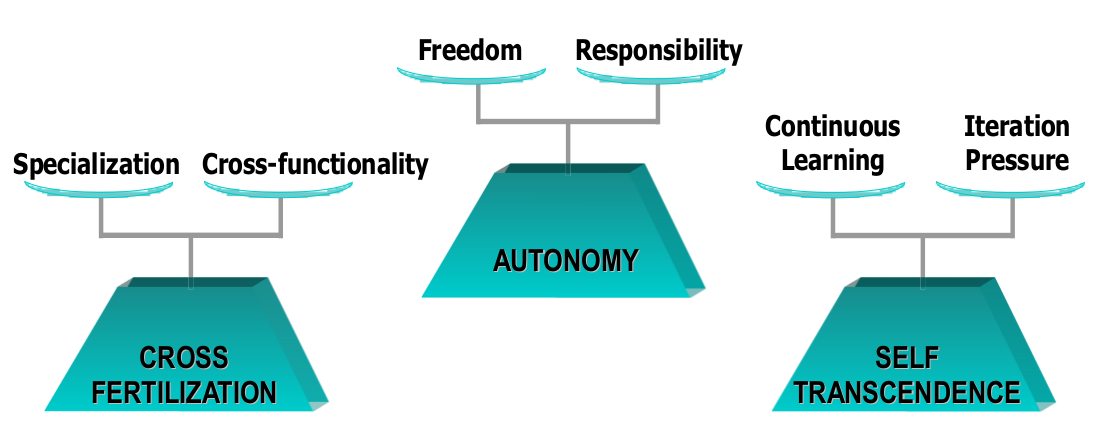
\includegraphics[width=0.5\textwidth]{balancing.png}   \caption{Relationship
between the Balancing Acts and the fundamental conditions of self-organisation
\cite{hoda2010balancing}.} \end{figure}

In a prescriptive software development process senior management is responsible
for setting the goals of the team. Managers assign tasks to specific team
members and perform evaluations of performance and productivity. This stems from
the hierarchical nature of traditional organizations and does not allow
developers to take ownership of the project on which they are working.

In contrast, Agile teams allow members to take ownership of the project on which
they are working by letting them guide development through Agile processes. This
requires Agile teams to be given freedom by upper management to take
responsibility for their project. By giving ownership of the project to the
team, senior management is encouraging members to have a greater sense of
responsibility for the project and hence be more motivated to produce higher
quality work.

With ownership of the project there also comes the freedom to make decisions
about that project, and the responsibility to make good decisions. Agile
facilitates this freedom through certain practices such as sprint planning,
the story board, and sprint retrospectives.

During sprint planning team members have the freedom to decide the direction of
the project for that iteration in terms of what features and work will be done.
The team also has the responsibility to not make a plan which is in the best
interests of the project rather than in their own best interests.

Team members also have the freedom to choose their own tasks from the story
board. Here team members have the freedom to practice autonomy by making their
own decisions about which tasks to pick up. The team must also act responsibly
and not choose only easy and low priority tasks from the task board. Fortunately
the transparent nature of the board discourages this through the social pressure
imposed by the need to meaningfully contribute.

The team also has the freedom to reflect and improve on their processes at the
sprint retrospective. Here the team must act responsibly by proactively
identifying their weaknesses and areas of improvement.

If members of a team fail to act responsibly it is the responsibility of senior
management or a Terminator \cite{hoda2010organizing} to identify those members
and discipline or remove from a team. This responsibility also requires
balancing as too much interference from management can jeopardise the ownership
a team feels towards their project \cite{hoda2010balancing}.

An Agile team must also balance its level of cross-fertilization. According to
Nonaka et al. cross fertilization requires a team to consist of members of
``varying functional specialisations'' which must interact and work together.
Ideally in an Agile team every member is a master of all trades, though
realistically there is some level of specialisation due to constraints on
resources and time.

The advantages of cross fertilization come when members cross-fertilize across
functional roles and cross technical areas of expertise
\cite{hoda2010balancing}.

By cross-fertilizing across functional roles teams can be more adaptive to a
changing workload and can cross barriers between functional specialisations. For
example, having a mix of functional roles can allow developers and testers to
work with one another, whereas when working separately they can often feel as
though they are working against one another.

Cross-fertilizing across technical areas of expertise allows for a greater
collective ownership of the project, which is in line with the XP principle of
collective code ownership \cite{beck1999embracing}. If multiple members of a
team are familiar with a technology then it increases the flexibility of the
team and helps members maintain an interest in their work.

Self-transcendence is the principle that teams establish their own goals and
practice continuous evaluation of themselves throughout a project. In Agile this
is achieved through the practices of sprint planning and sprint retrospectives.
Through this practice teams must balance the amount of iteration pressure with
the level of continuous learning \cite{hoda2010balancing}.

Iteration pressure is the pressure induced by time restrictions during a sprint.
While some iteration pressure is desirable as a motivating factor, too much
iteration pressure causes teams to eat into time that could be more productively
spent practising continuous learning. Continuous learning is important for a
team to remain flexible and keep innovating.

\subsection{Roles}

Through a Grounded Theory \cite{strauss1994grounded} study conducted using 24
Agile practitioners in 14 different software organisations in New Zealand and
India, six informal roles were consistently adopted by members of Agile teams
\cite{hoda2010organizing}.

The \emph{mentor} role is played by a member who guides the team through the use
of Agile processes. Despite the simplicity of Agile processes, practising Agile
can be difficult. The Mentor encourages the team to learn and adhere to Agile
practices.

The \emph{co-ordinator} acts as a liaison between the team and the customer. The
co-ordinator gathers initial requirements from the customer and communicates any
changes the customer requires. The co-ordinator is especially important for
teams which are servicing an offshore customer \cite{hoda2010organizing}, as it
is impractical for the entire team to maintain close contact with a customer
which is overseas.

The \emph{translator}



\section{Project Experience}

The project we undertook from Orion Health was a streamlined check in system
which we dubbed ``Vital Stats Manager'' or ``VSM'' which is intended to replace
paper forms when arriving at a hospital check in. The system consists of four
major components, three of which we tackled over four sprints. These components
are the VSM Android Application, the VSM NFC Receiver, the VSM Server and API,
and the VSM Web Application.

The VSM Android Application is intended to be distributed and installed on
patient's Android devices. It consists of a form which replaces the paper form
normally filled out when checking in to a hospital. This form allows patients to
enter their vital medical information, such as their height, weight, allergies,
etc.

The VSM NFC Receiver is the component of the system which was not fully
developed over the four sprints of the project due to limitations in the
availability of required NFC hardware. For the purposes of the project a mock
receiver was developed as an Android application, though the user interface was
not a focus. The role of this component is to receive patient check ins. At the
reception of each hospital department it is envisioned that there will be one of
these receivers which a patient can touch with their Android device with the VSM
Android Application installed. By touching the receiver they transmit their
vital information to the hospital and are checked in.

The VSM Server and API component is the component which receives, stores, and
exposes patient check ins. When a patient checks in by transmitting their vital
information over NFC to the receiver, the receiver uploads the received data to
the server which stores it in a database. This information is then exposed via a
RESTful API for consumption by other components of the system.

The VSM Web Application is the main consumer of the data exposed by the VSM
Server and API. It is intended that receptionists and nurses can see recent
check ins to a department and review and edit patient vital information as
patients check in to the hospital. It provides functions to search, filter, edit
and delete patients.

The team for this project consisted of six members; myself, Michael Little,
Jourdan Harvey, Dave Carpenter, Andrew Luey, and Thomas Lugnet. This team was
self assembled before the project requirements were available. Each member was
familiar with the others and had differing degrees of software development
experience.

After receiving the project description and before our first meeting with our
customer representatives we decided to work on a prototype of the system based
on our understanding of the requirements. This gave the team an opportunity to
research and familiarize themselves with the technologies which would be used to
develop the final working system.

At our first meeting with our customer representatives we clarified the project
requirements and realised our understanding was not complete. Fortunately our
prototypes of the system components were modifiable to the point where this was
not a large concern and our technology choices were not affected. Here we see an
example of the way Agile teams can react more easily to changes in requirements,
due to the short iterations and frequent customer interaction our software was
able to adapt easily.

After gathering the requirements from our first meeting with our customer
representatives we self organised into pairs roughly mapping to the three
components which we were to implement. Particular members of our team had more
experience in different areas of development. This was important with regard to
the manner in which we self organised. Dave and myself had experience in back
end development relevant to the Server and API, Michael had experience in
Android development, and Dave, Jourdan and I had experience in web front end
development.

To encourage our team members to become ``masters of all trades'' and avoid too
much specialisation we organised pairs so that a member with experience in the
area of the system they were developing was paired with a member with less or no
experience in that area. By practising pair programming members were able to
learn about the technologies and the implementation details of the part of the
system on which they were working. In this manner we avoided any one team member
becoming a specialist, though there was a certain level of skill segregation
amongst the team. This can be attributed to the time constraints of the project
and the need to learn new technologies. We were unable to sacrifice the time to
let all users spend time learning each of the myriad technologies employed
across the three components of our system.

Three pairs ended up forming - myself and Andrew Luey worked on the VSM Server
and API. I had experience in developing RESTful APIs backed by databases similar
to the way this component was going to work. Michael had previous Android
development experience and so Jourdan and Michael worked on the VSM Android
Application. Dave had some limited experience in web development and so Dave and
Thomas worked on the VSM Web Application.

Despite certain members having relevant experience, the specific technologies we
chose were not necessarily familiar. Those members with experience could more
easily pick up these new technologies and therefore expedite the learning of
those less experienced members. For example, we used an ORM called SQLAlchemy to
interface with our database in the VSM Server component. I was able to quickly
pick up this technology from my previous experience with different ORMs and in
the process teach Luey the important aspects necessary for the development of
our system.

Over the development of the project we had roughly weekly meetings with our
customer representatives from Orion Health - that is two meetings per sprint. As
Agile practitioners themselves they acted as mentors as well as customers.

In their role as mentors they advocated certain Agile practices to us -
especially test driven development. We managed to incorporate this technique
more and more as our software stabilised and we became more familiar with the
technologies we were using.

As customers our representatives at Orion provided us with the requirements for
the project. As the project progressed and we completed the original user
stories and met milestones they would add requirements to the project. Here we
see another example of Agile methodologies and the way requirements can change
and planning can occur at late stages of the project, as opposed to more
prescriptive methodologies in which changes may be more difficult to
incorporate.

Some examples of late requirements added by our customers were the additions of
department log ons and breadcrumbs. The customers asked for the ability to
separate patients by departments and let nurses and administrative staff see
only those patients from specific departments. This requirement was added in the
fourth sprint of the project after we had become familiar with our code and the
technologies we were using. This gave us an opportunity to practice TDD. The
main change had to occur in the server where we needed to change the way
patients were accessed to limit them to departments. We were able to add tests
which would verify the correctness of our implementation and then implement the
changes. From this we saw the value of the red-green-refactor cycle.

The second requirement - the addition of breadcrumbs to the web interface - was
also introduced in the fourth sprint. At this point we were able to become more
cross functional as a team as we had overcome the learning phase. As a result I
was able to work on this requirement which was outside of the VSM Server
component I had been mainly responsible for up to this point. Given more time I
can see how this could have occurred in other places with other members as work
would run out in specific areas and members would be required to undertake tasks
in unfamiliar areas of the code base.

The tool we used throughout development for organising work was GitHub. GitHub
acts as a source control repository and issue tracker. The issue tracker allowed
us to add tasks to certain milestones and assign them to members. It also
allowed us to implement code reviews through a feature called ``pull requests.''

The issue tracker was used as the mechanism for which work was distributed
throughout the team. At the beginning of an iteration after our sprint planning
and retrospective we would create issues which represented the tasks which we
intended to complete in that iteration. These tasks were then available to be
picked up by any member who wished to undertake them. Issues were also logged as
development occurred and new requirements were recognised or bugs found. For
example, while developing the NFC Receiver which would upload patient
information to the server, Michael and Jourdan would identify bugs and issues
they had with the RESTful API. By logging these on GitHub everyone would receive
an email with the bug report, allowing anyone to pick up and comment on the bug.

``Pull requests'' are the key feature of GitHub which democratise code reviews.
Whenever a feature or bug fix was finished on a branch, a member could open a
pull request, requesting their code be integrated into the master branch.
Members would then receive an email detailing the code changes and are able to
discuss the changes, comment on specific lines of code, add their own commits to
the changes, and eventually approve the pull request for merging. GitHub
themselves uses these features to practice self-organization and code review
{REF}.


\section{Discussion}


\section{Implications for Practice}


\section{Conclusion}


\section*{Acknowledgement}


\bibliographystyle{IEEEtran}
\bibliography{essay}


\end{document}
